\documentclass[aspectratio=169]{../latex_main/tntbeamer}  % you can pass all options of the beamer class, e.g., 'handout' or 'aspectratio=43'
\usepackage{dsfont}
\usepackage{bm}
\usepackage[english]{babel}
\usepackage[T1]{fontenc}
%\usepackage[utf8]{inputenc}
\usepackage{graphicx}
\graphicspath{ {./figures/} }
\usepackage{algorithm}
\usepackage[ruled,vlined,algo2e,linesnumbered]{algorithm2e}
\usepackage{hyperref}
\usepackage{booktabs}
\usepackage{mathtools}

\usepackage{amsmath,amssymb}

\DeclareMathOperator*{\argmax}{arg\,max}
\DeclareMathOperator*{\argmin}{arg\,min}

\usepackage{amsbsy}
\newcommand{\vect}[1]{\bm{#1}}
%\newcommand{\vect}[1]{\boldsymbol{#1}}

\usepackage{pgfplots}
\pgfplotsset{compat=1.16}
\usepackage{tikz}
\usetikzlibrary{trees} 
\usetikzlibrary{shapes.geometric}
\usetikzlibrary{positioning,shapes,shadows,arrows,calc,mindmap}
\usetikzlibrary{positioning,fadings,through}
\usetikzlibrary{decorations.pathreplacing}
\usetikzlibrary{intersections}
\pgfdeclarelayer{background}
\pgfdeclarelayer{foreground}
\pgfsetlayers{background,main,foreground}
\tikzstyle{activity}=[rectangle, draw=black, rounded corners, text centered, text width=8em]
\tikzstyle{data}=[rectangle, draw=black, text centered, text width=8em]
\tikzstyle{myarrow}=[->, thick, draw=black]

% Define the layers to draw the diagram
\pgfdeclarelayer{background}
\pgfdeclarelayer{foreground}
\pgfsetlayers{background,main,foreground}

% Requires XeLaTeX or LuaLaTeX
%\usepackage{unicode-math}

\usepackage{fontspec}
%\setsansfont{Arial}
\setsansfont{RotisSansSerifStd}[ 
Path=../latex_main/fonts/,
Extension = .otf,
UprightFont = *-Regular,  % or *-Light
BoldFont = *-ExtraBold,  % or *-Bold
ItalicFont = *-Italic
]
\setmonofont{Cascadia Mono}[
Scale=0.8
]

% scale factor adapted; mathrm font added (Benjamin Spitschan @TNT, 2021-06-01)
%\setmathfont[Scale=1.05]{Libertinus Math}
%\setmathrm[Scale=1.05]{Libertinus Math}

% other available math fonts are (not exhaustive)
% Latin Modern Math
% XITS Math
% Libertinus Math
% Asana Math
% Fira Math
% TeX Gyre Pagella Math
% TeX Gyre Bonum Math
% TeX Gyre Schola Math
% TeX Gyre Termes Math

% Literature References
\newcommand{\lit}[2]{\href{#2}{\footnotesize\color{black!60}[#1]}}

%%% Beamer Customization
%----------------------------------------------------------------------
% (Don't) Show sections in frame header. Options: 'sections', 'sections light', empty
\setbeamertemplate{headline}{empty}

% Add header logo for normal frames
\setheaderimage{
	% 
\includegraphics[height=\logoheight]{figures/TNT_darkv4.pdf}
	
\includegraphics[height=\logoheight]{../latex_main/figures/luh_logo_rgb_0_80_155.pdf}
	% 
\includegraphics[height=\logoheight]{figures/logo_tntluh.pdf}
}

% Header logo for title page
\settitleheaderimage{
	% 
\includegraphics[height=\logoheight]{figures/TNT_darkv4.pdf}
	
\includegraphics[height=\logoheight]{../latex_main/figures/luh_logo_rgb_0_80_155.pdf}
	% 
\includegraphics[height=\logoheight]{figures/logo_tntluh.pdf}
}

% Title page: tntdefault 
\setbeamertemplate{title page}[tntdefault]  % or luhstyle
% Add optional title image here
%\addtitlepageimagedefault{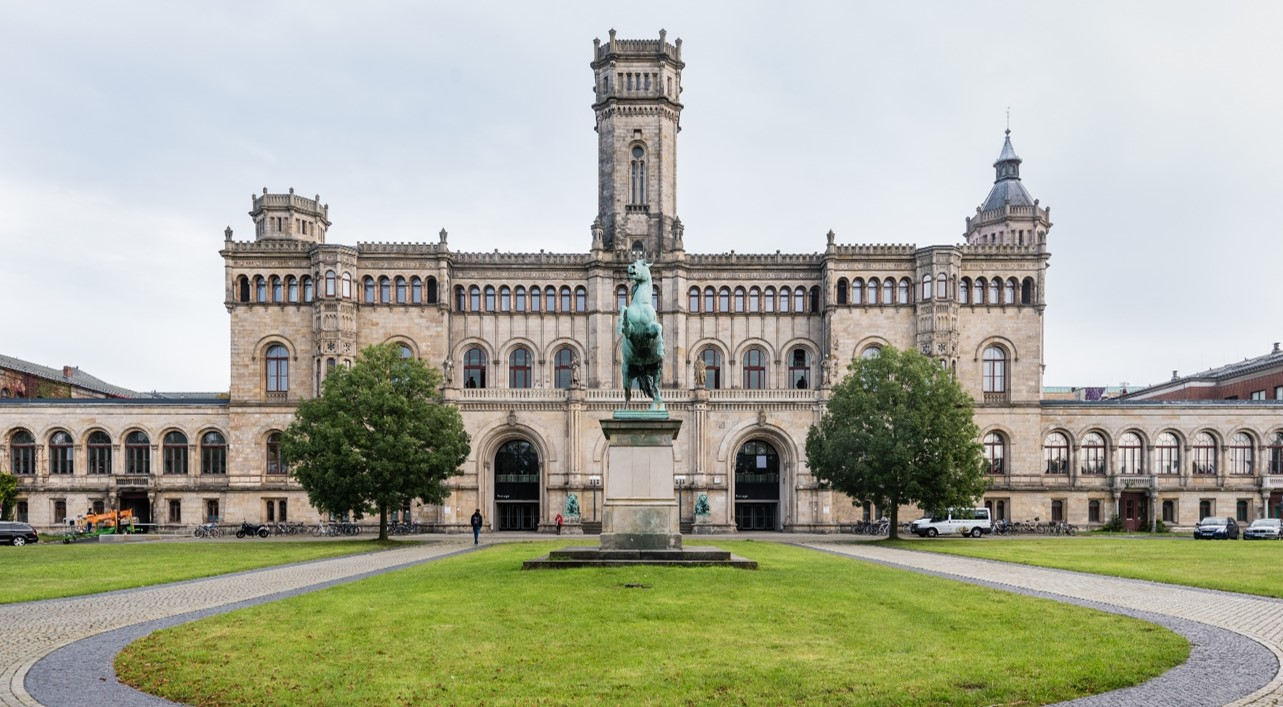
\includegraphics[width=0.65\textwidth]{figures/luh_default_presentation_title_image.jpg}}

% Title page: luhstyle
% \setbeamertemplate{title page}[luhstyle]
% % Add optional title image here
% \addtitlepageimage{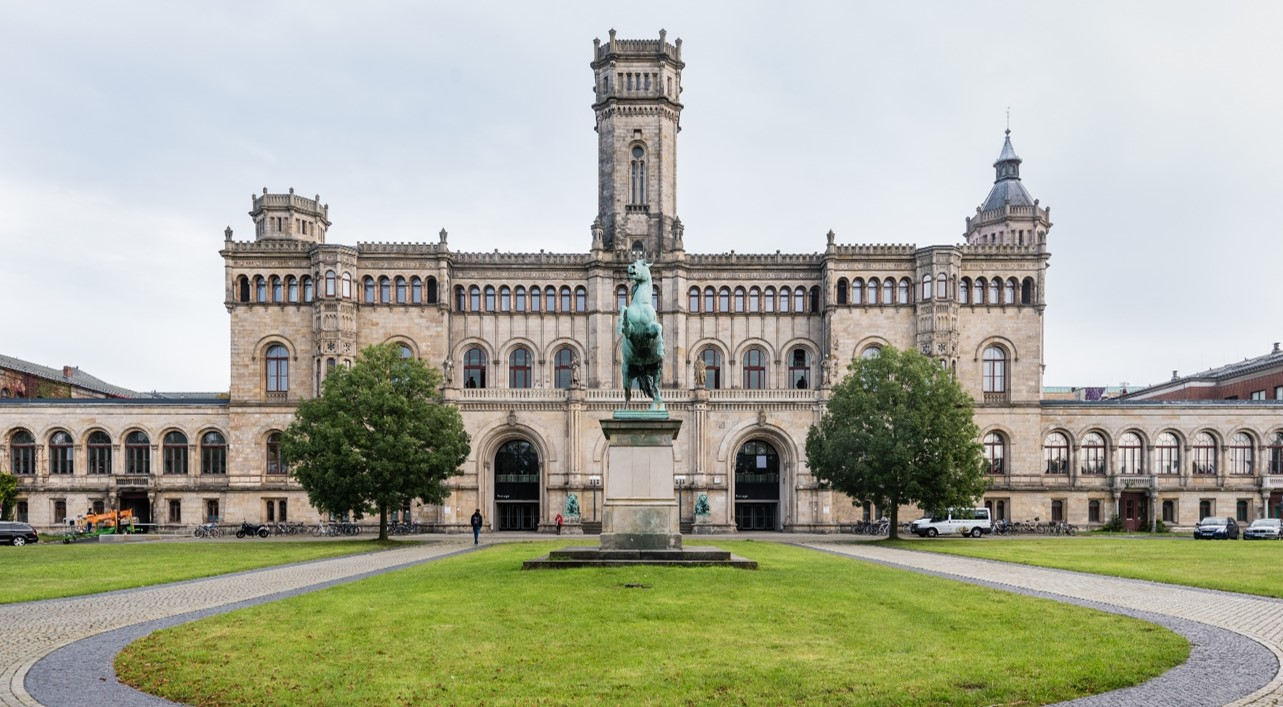
\includegraphics[width=0.75\textwidth]{figures/luh_default_presentation_title_image.jpg}}

\author[Abedjan \& Lindauer]{Ziawasch Abedjan \& Marius Lindauer\\[1em]
	
\includegraphics[height=\logoheight]{../latex_main/figures/luh_logo_rgb_0_80_155.pdf}\qquad
	
\includegraphics[height=\logoheight]{../latex_main/figures/DBIS_Kurzlogo.png}\qquad

\includegraphics[height=\logoheight]{../latex_main/figures/TNT_darkv4}\qquad

\includegraphics[height=\logoheight]{../latex_main/figures/L3S.jpg}	}
\date{Summer Term 2022; \hspace{0.5em} {
\includegraphics[height=1.5em]{../latex_main/figures/Cc-by-nc-sa_icon.svg.png}}; based on \href{https://ds100.org/fa21/}{[DS100]}
}


%%% Custom Packages
%----------------------------------------------------------------------
% Create dummy content
\usepackage{blindtext}

% Adds a frame with the current page layout. Just call \layout inside of a frame.
\usepackage{layout}


%%% Macros
%\renewcommand{\vec}[1]{\mathbf{#1}}
% \usepackage{bm}
%\let\vecb\bm

\title[Introduction]{DS: Logistic Regression, Part 1}
\subtitle{Maximum likelihood estimation}

\graphicspath{ {./figure/} }
%\institute{}


\begin{document}
	
	\maketitle
	\begin{frame}{Where did log loss come from?}
	    Log loss seemed to have come out of thin air.
	    \begin{itemize}
	        \item It seems to make a lot of sense for a model that predicts probabilities!
	        \item Let’s derive where it came from.
	    \end{itemize}
	\end{frame}
	
	
	
	\begin{frame}{Estimating the chance of success}
	    Suppose I have a coin that flips heads with probability p. Assume each flip is independent.
	    \begin{itemize}
	        \item I don’t know what p is, but I flip the coin 10 times and I see 0001011001 (4 heads, 6 tails).
	        \item Can model each flip with an i.i.d. Bernoulli(p) random variable (1 for heads, 0 for tails).
	        \item What is the most likely value of p?
	    \end{itemize}
	    \begin{equation*}
	        L(p) = p^4(1-p)^6
	    \end{equation*}
	    This function is called the likelihood of our observed sequence.
	    \begin{figure}
	        \centering
	        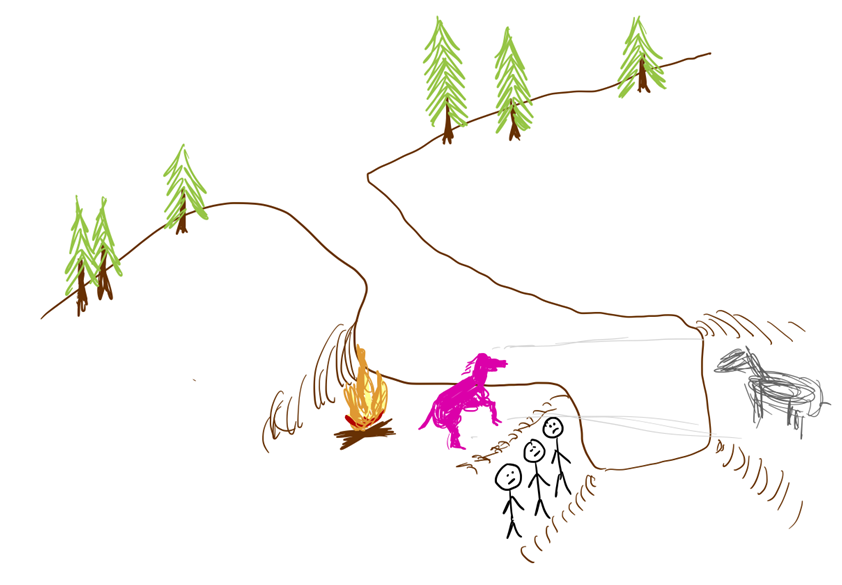
\includegraphics[scale=.75]{Bild24}
	    \end{figure}
	\end{frame}
	
	
	\begin{frame}{Estimating the chance of success}
	    Suppose I have a coin that flips heads with probability p. Assume each flip is independent.
	    \begin{itemize}
	        \item I don’t know what p is, but I flip the coin 10 times and I see 0001011001 (4 heads, 6 tails).
	        \item Can model each flip with an i.i.d. Bernoulli(p) random variable (1 for heads, 0 for tails).
	        \item What is the most likely value of p?
	    \end{itemize}
	    \begin{equation*}
	        L(p) = p^4(1-p)^6
	    \end{equation*}
	    This function is called the likelihood of our observed sequence.
	    \begin{columns}
	        \begin{column}{.5\textwidth}
	        \\
	        \bigskip
	                We’d estimate  $\hat{p}$   = 0.4.
                \begin{itemize}
                    \item Sample proportion of 1s.
                    \item Maximizes likelihood function over all p. 
                \end{itemize}
	        \end{column}
	        
	        
	        \begin{column}{.4\textwidth}
	               \begin{figure}
	                     \centering
	                     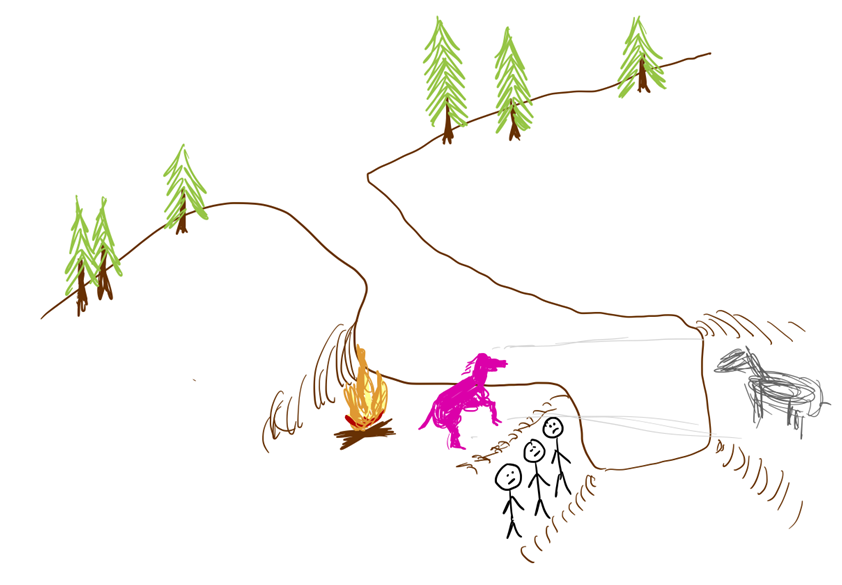
\includegraphics[scale=.7]{Bild24}
	              \end{figure}
	        \end{column}
	        
	        
	    \end{columns}
	    
	\end{frame}
	
	
	
	\begin{frame}{Two different coins}
	   \begin{itemize}
	       \item Toss a coin that lands heads with chance p1.
	       \begin{itemize}
	           \item Result: Y1.
	       \end{itemize}
	       \item Toss a coin that lands heads with chance p2.
	       \begin{itemize}
	           \item Result: Y2.
	       \end{itemize}
	       \item What are the probabilities for all possible combinations of values?
	   \end{itemize}
	   
	   $P(Y_1 = 1,Y_2 = 1) = p_1p_2$\\
	   $P(Y_1 = 1,Y_2 = 0) = p_1(1-p_2)$\\
	   $P(Y_1 = 0,Y_2 = 1) = (1 - p_1)p_2$\\
	   $P(Y_1 = 0,Y_2 = 0) = (1 - p_1)(1 - p_2)$
	\end{frame}
	
	
	\begin{frame}{PMF of the Bernoulli distribution}
	   If Y is the result of one toss of a coin that lands heads with chance p,
	   \begin{align*}
	       P(Y = y) & = \left\{\begin{array}{cc}
	           p & \text{if } y = 1 \\
	          1-p   & \text{if } y = 0
	       \end{array}\right.\\
	       &= p^y(1-p)^{1-y}
	   \end{align*}
	   We’ve seen the first form already. Why are they equivalent?\\
	   Then, if Y1 and Y2 are the results of tosses of two coins:
	   \begin{equation*}
	       P(Y_1 = y_1, Y_2 = y_2) = (p_1^{y_1}(1- p_1)^{1-y_1})(p_2^{y_2}(1 - p_2)^{1 -y_2})
	   \end{equation*}
	   
	\end{frame}
	
	
	\begin{frame}{Estimating the two probabilities}
	   \begin{itemize}
	       \item Suppose we want to estimate the values of p1 and p2.
	       \item We know what the likelihood is.
	   \begin{equation*}
	       P(Y_1 = y_1, Y_2 = y_2) = (p_1^{y_1}(1- p_1)^{1-y_1})(p_2^{y_2}(1 - p_2)^{1 -y_2})
	   \end{equation*}
	   \item Our goal is to find the $\hat{p_1}$ and$\hat{p_2}$ that maximize the above function, over all p1 and p2.
	   \begin{itemize}
	       \item Maximize, because we are looking for the p1 and p2 that are “most likely” to have generated the data that we observed.
	   \end{itemize}
	   \item As before, this involves differentiating, setting equal to 0, and solving.
	   \end{itemize}
	\end{frame}
	
	
	
	\begin{frame}{Log likelihoods}
	   \begin{itemize}
	       \item Maximizing     $P(Y_1 = y_1, Y_2 = y_2) = (p_1^{y_1}(1- p_1)^{1-y_1})(p_2^{y_2}(1 - p_2)^{1 -y_2})$ is annoying. 
	       \begin{itemize}
	           \item Products -> chain rule.
	       \end{itemize}
	   \item log(x) is a strictly increasing function.
	   \begin{itemize}
	       \item If a > b, then log(a) > log(b).
	   \end{itemize}
	   \item This means, the values of p1 and p2 that maximize      $P(Y_1 = y_1, Y_2 =y_2)$                           are the same values that maximize
	   \end{itemize}
	   \begin{align*}
	        &\log ((p_1^{y_1}(1- p_1)^{1-y_1})(p_2^{y_2}(1 - p_2)^{1 -y_2}))\\
	        &= y_1\log(p_1) + (1 - y_1)\log(1-p_1) + y_2\log (p_2) + (1 - y_2)\log(1-p_2)\\
	        &= \sum\limits_{i=1}^2(y_i\log(p_i) + (1 - y_i)\log(1-p_i))
	   \end{align*}
	   Starting to look familiar!

	\end{frame}
	
	
	\begin{frame}{Estimating n probabilities}
	   \begin{itemize}
	       \item For i = 1, 2, …, n, let $Y_i$ be Bernoulli($p_i$).
	       \begin{itemize}
	           \item Each $Y_i$ is independent of each other.
	       \end{itemize}
	   \item To estimate          $p_1, p_2, \dots,p_n$                  :
	   \begin{itemize}
	       \item If a > b, then log(a) > log(b).
	   \end{itemize}
	   \item This means, the values of p1 and p2 that maximize      $P(Y_1 = y_1, Y_2 =y_2)$                           are the same values that maximize
	   \end{itemize}
	   \begin{align*}
	       \text{Find } \hat{p}_1, \hat{p}_2, \dots, \hat{p}_n\text{that maximize } \sum\limits_{i=1}^n(y_i\log(p_i) + (1 - y_i)\log(1-p_i))
	   \end{align*}
	   Equivalently:
	   \begin{equation*}
	       \text{Find } \hat{p}_1, \hat{p}_2, \dots, \hat{p}_n\text{that minimize } -\frac{1}{n}\sum\limits_{i=1}^n(y_i\log(p_i) + (1 - y_i)\log(1-p_i))
	   \end{equation*}
        We choose this equivalent form because we are more used to minimizing loss.

	\end{frame}
	
	
	\begin{frame}{Cross-entropy loss}


	   \begin{equation*}
	       \text{Find } \hat{p}_1, \hat{p}_2, \dots, \hat{p}_n\text{that minimize } -\frac{1}{n}\sum\limits_{i=1}^n(y_i\log(p_i) + (1 - y_i)\log(1-p_i))
	   \end{equation*}
   	    What does this have to do with logistic regression?
   	    \begin{itemize}
   	        \item We have n observations (y1, y2, …, yn). Each is either 1 or 0.
   	        \begin{itemize}
   	            \item Assume that each is independent of one another.
   	        \end{itemize}
   	        \item Can think of observation $y_i$ as the result of a coin toss with probability pi.
   	        \begin{itemize}
   	            \item The output of our logistic regression model is our estimate for the probability that     $y_i$ = 1.
   	            \item Thus, we can use the above average loss, with  $p_i = \sigma (\mathbb{X}_i^T\theta)$.
   	            \item This gives us the exact same expression for cross-entropy loss that we saw before!
   	        \end{itemize}
   	    \end{itemize}

	\end{frame}
	
	
	\begin{frame}{Maximum likelihood estimation}

        Minimizing cross-entropy loss is equivalent to maximizing the likelihood of the data.
   	    \begin{itemize}
   	        \item We are choosing the model parameters that are “most likely”, given this data.
   	        \item Another perspective of fitting our model to the data.
   	        \begin{equation*}
   	            R(\theta) = -\frac{1}{n}\sum\limits_{i=1}^n(y_i\log(\sigma (\mathbb{X}_i^T\theta)) + (1 - y_i)\log(1-\sigma (\mathbb{X}_i^T\theta)))
   	        \end{equation*}
   	    \end{itemize}
        This technique is called maximum likelihood estimation (MLE).
        \begin{itemize}
            \item It turns out, many of the model + loss combinations we’ve seen in this class can be motivated using MLE.
            \begin{itemize}
                \item OLS, Ridge Regression.
            \end{itemize}
            \item You will study this further in probability and ML classes. But now you know it exists.
        \end{itemize}
	\end{frame}
\end{document}